\newpage
\section{Introduction to Transaction Processing Concepts and Theory}


% Introduzione alle transazioni
\subsection{Introduzione alle transazioni}

Il concetto di transazione è in \hl{contrapposizione con il concetto di query} dato che:

\begin{itemize}
    \item query: esecuzione di iscruzioni per ottenere delle informazioni
    \item \hl{transazione}: \textbf{descrive l'unità di elaborazione del DB} cioè un insieme di query con 2 stadi fissi (inizio e fine)
\end{itemize}

Ci troveremo in un \hl{sistema transazionale} se ho 2 \hl{utenti concorrenti} (multiuser DBMS) che vogliono accedere allo stesso DB. Quindi se avrò dei DB molto ampi, con centinauia di possibili utenti che vogliono accedervi contemporaneamente dovrò avere 2 \hl{requisiti} prestazionali:

\begin{itemize}
    \item alta \textbf{disponibilità}
    \item alta \textbf{velocità di risposta}
\end{itemize}

oppure posso usare il \hl{multiprogramming} consentendo al OS di mandare in esecuzione istruzioni di più processi in parallelo o in interleaved (interlacciato).


\begin{figure}[H]
\centering
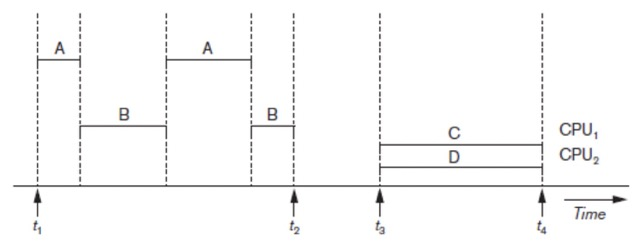
\includegraphics[scale=0.4]{multiuser.jpeg}
\caption{Processo paralleo e interleaved} 
\label{multiuser}
\end{figure}


I \hl{tipi di transazione} che possiamo avere sono in:

\begin{itemize}
    \item sola lettura
    \item lettura e scrittura
\end{itemize}

e possono avvenire su item, record, attributi di un database, o anche su un blocco del disco. Quando si eseguono queste operazioni, i \hl{buffer vengono salvati nel DBMS} che una volta pieni vengono sostituiti tramite il \hl{last recently used}. Tutto ciò \hl{indipendentemente dalla granularita' dell'item}, con notazione:

\begin{lstlisting}
operazione_item(x)
\end{lstlisting}

e chiamaremo:

\begin{itemize}
    \item \textbf{read set}: tutto quello letto in una transazione
    \item \textbf{write set}: tutto quello scritto in una transazione 
\end{itemize}


\begin{figure}[H]
\centering
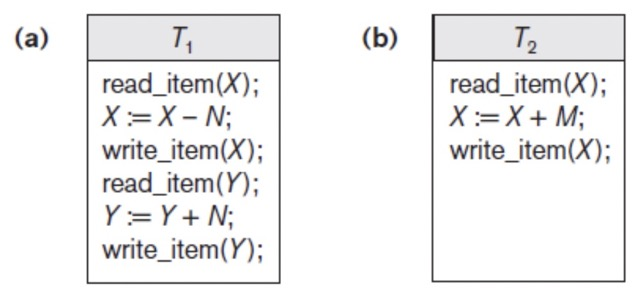
\includegraphics[scale=0.4]{2trans.jpeg}
\caption{Due transazioni indipendenti} 
\label{2trans}
\end{figure}


% Problemi durante le transazioni
\subsection{Problemi durante le transazioni}

Possono essere:

\begin{itemize}
    \item \hl{lost update}: quando le \textbf{esecuzioni della transazione $i$ sono interleaved con la $i+1$}
   

    \begin{figure}[H]
    \centering
    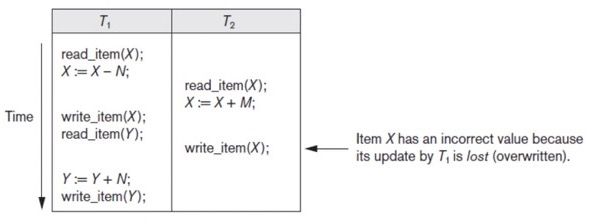
\includegraphics[scale=0.4]{lostupdate.jpeg}
    \caption{Lost Update Problem} 
    \label{lostupdate}
    \end{figure}

    con $T_2$ che legge il valore originale e l'aggiornamento di $T_1$ viene sovrascritto a quello di $T_2$
    
    
    \item \hl{temporary update (dirty read)}: quando una transazione accede ad un dato e poi fallisce e nello stesso tempo un'altra accede allo stesso dato, questa \textbf{continua a leggere il valore della transazione fallista} (dirty data)
    
    \begin{figure}[H]
    \centering
    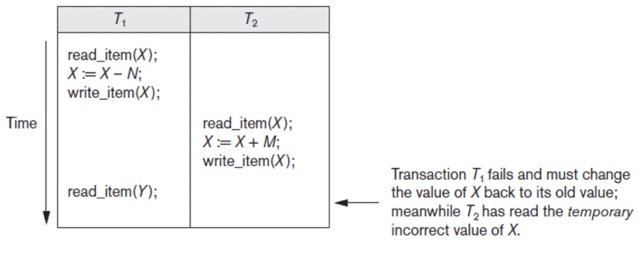
\includegraphics[scale=0.4]{dirtyread.jpeg}
    \caption{Dirty Read Problem} 
    \label{dirtyread}
    \end{figure}


    \item \hl{incorrect summary}: quando cerco di accedere a dei dati che stanno essendo modificati \textbf{leggendo alcuni dati già modificati e altro no}
    
    \begin{figure}[H]
    \centering
    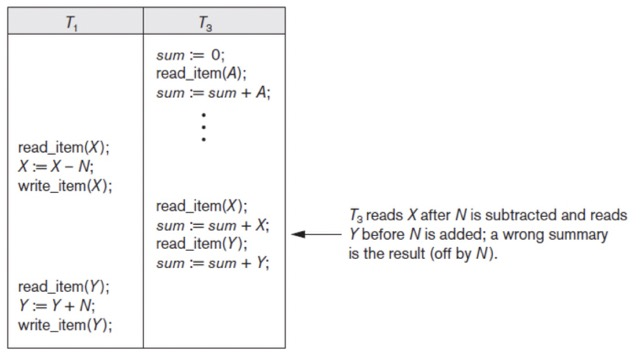
\includegraphics[scale=0.4]{incsum.jpeg}
    \caption{Incorrect Summary Problem} 
    \label{incsum}
    \end{figure}


    \item \hl{unrepeatable read}: quando si effettua una \textbf{lettura doppia del dato} ma il \textbf{valore della funzione ripetuta} ad intervalli di tempo differenti \textbf{e' diversa}
\end{itemize}


% Le operazioni di una transazione
\subsection{Le operazioni di una transazione}

Possono essere:

\begin{itemize}
    \item \hl{BEGIN\_TRANSACTION}: fa iniziare la transazione
    \item \hl{READ or WRITE}: operazioni di lettura o scirttura sul DB
    \item \hl{END\_TRANSACTION}: segna la fine della transazione e delle operazioni di lettura/scrittura. fa anche un \textbf{check sui cambiamente effettuati} come può essere l'interleaved
    \item \hl{COMMIT\_TRANSACTION}: segnala una \textbf{fine con successo} e l'invio del commit delle transazioni, ottenendo un \textbf{commit point} che affiancato all'Id della transazione mi permette di capire queli di queste sono fallite
    \item \hl{ROLLBACK}: segnala un \textbf{fail della transazione} e quindi la successiva \textbf{cancellazione dei cambiamenti}
\end{itemize}

\begin{figure}[H]
\centering
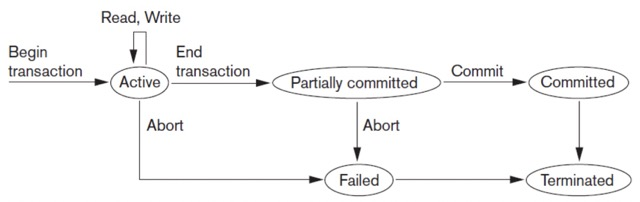
\includegraphics[scale=0.4]{opertrans.jpeg}
\caption{Operazioni delle transazioni} 
\label{opertrans}
\end{figure}


% Proprietà delle transazioni
\subsection{Proprietà delle transazioni}

Le proprietà fondamentali per ogni transazione sono dette \hl{ACID}:

\begin{itemize}
    \item \hl{Atomicity}: dove o \textbf{esegui la transazione intera} o non la esegui
    \item \hl{Consistency}: quando la transazione termina \textbf{non lascia inconsistenza}
    \item \hl{Isolation}: dove la transazione \textbf{non interferisce} con altre transazioni
    \item \hl{Durability/permanency}: dalla transazione devo avere delle \textbf{modifiche permamnenti nel DB}
\end{itemize}


% Scheduling basato sulla recoverability
\subsection{Scheduling basato sulla recoverability}

Lo scheduling \hl{contiente}:

\begin{itemize}
    \item \textbf{ordine di esecuzione delle operazioni} da tutte le transazioni
    \item operazioni di \textbf{transazioni diverse}
\end{itemize}

Potremo avere due \hl{operazioni in conflitto} se:

\begin{itemize}
    \item appartengono a \textbf{transazioni diverse}
    \item accedono allo \textbf{stesso elemento $X$}
    \item ha un'operazione di \textbf{write}
\end{itemize}



% La serializzazione
\subsection{La serializzazione}

È importante perché \hl{non permette l'interleaved} tra le transazioni, eliminando i problemi sopra citati. Se presa \hl{come unica risorsa non e' realizzabile}, allora ci si chiede quali siano le schcedulazioni che si posso serializzare (solo $n$ transazioni).
